\documentclass[a4paper,ngerman,12pt]{scrartcl}

\usepackage[utf8]{inputenc}
%\usepackage[ansinew]{inputenc}

\usepackage[ngerman]{babel}

\usepackage{amsmath,amsthm,amssymb,mathtools,stmaryrd,color,graphicx}
\usepackage{setspace}
\usepackage{bussproofs}
\usepackage{array}
\usepackage{comment}
\usepackage{wrapfig}

\usepackage{enumitem}

\usepackage{units}

\usepackage[protrusion=true,expansion=true]{microtype}

\usepackage{lmodern}

\usepackage{hyperref}
\usepackage{cleveref}

\newcommand{\IR}{\mathbb{R}}
\newcommand{\IC}{\mathbb{C}}
\newcommand{\IZ}{\mathbb{Z}}
\newcommand{\IN}{\mathbb{N}}
\newcommand{\IQ}{\mathbb{Q}}

\setlength\parskip{\medskipamount}
\setlength\parindent{0pt}

\theoremstyle{definition}
\newtheorem{defn}{Definition}[]
\newtheorem{axiom}[defn]{Axiom}
\newtheorem{bsp}[defn]{Beispiel}

\RequirePackage{framed}
\newtheorem{aufg}{Aufgabe}
\definecolor{shadecolor}{rgb}{.96,.96,.96}
\newenvironment{aufgabe}[1][]
		{\begin{shaded}\vspace{-0.3cm}\begin{aufg}\emph{#1} \par\medskip}
		{\end{aufg}\vspace{-0.3cm}\end{shaded}}
\newtheorem{zaufg}{Zusatzaufgabe}
	
\newenvironment{spiel}[1][]{\begin{framed}\textbf{#1:}\\}{\end{framed}}


\theoremstyle{plain}
\newtheorem{prop}[defn]{Proposition}
\newtheorem{motto}[defn]{Motto}
\newtheorem{wunder}[defn]{Wunder}
\newtheorem{ueberlegung}[defn]{Überlegung}
\newtheorem{lemma}[defn]{Lemma}
\newtheorem{kor}[defn]{Korollar}
\newtheorem{hilfsaussage}[defn]{Hilfsaussage}
\newtheorem{satz}[defn]{Satz}
\newtheorem{frage}[defn]{Frage}

\theoremstyle{remark}
\newtheorem{bem}[defn]{Bemerkung}
\newtheorem{beob}[defn]{Beobachtung}

	
\newtheorem*{antwort}{Antwort}

%\newlength{\aufgabenskip}
%\setlength{\aufgabenskip}{1.4em}
%\newcounter{aufgabennummer}
%\newenvironment{aufgabe}[1]{
%	\addtocounter{aufgabennummer}{1}
%	\textbf{Aufgabe \theaufgabennummer.} \emph{#1} \par
%}{\vspace{\aufgabenskip}}

\clubpenalty=10000
\widowpenalty=10000
\displaywidowpenalty=10000

\setlength\unitlength{1cm}

\usepackage{tikz}
\usetikzlibrary{calc}
\usepackage{tkz-euclide}
\usepackage{adjustbox}
\usepackage{algorithm2e}
\usepackage{pgfplots}

\RequirePackage{geometry}
\geometry{textwidth=17.0cm,textheight=25cm,footskip=1.5cm}


\newcommand{\kante}[2]{#1{-}#2}
\newcommand{\edge}[3]{\draw[thick] (#1) --node[rectangle,fill=gray!10]{$#3$} (#2);}

\begin{document}
	
\begin{picture}(0,0)
\put(0,-0.5){%
	
\includegraphics[scale=0.1]{logo-ifm}
}
\put(14.0,-3.5){%
	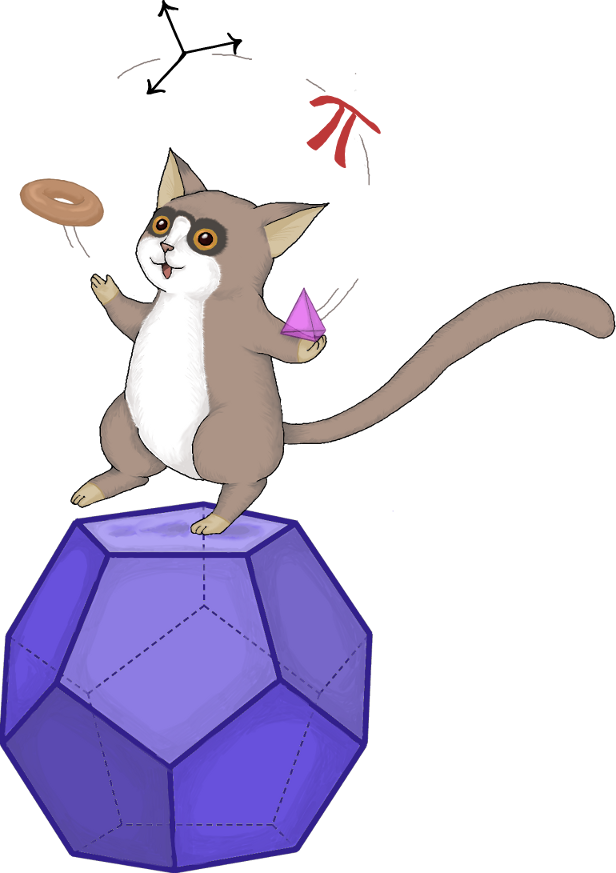
\includegraphics[scale=0.17]{cover}
}
\end{picture} 
	
\vspace{6em}

\begin{center}\Large{Mathe-Camp 2023}

\section*{Planare Graphen}\end{center}

\begin{aufg}
	In dem folgenden Bild siehst du zwei Wohnhäuser und drei Fabriken, die Wasser (W), Gas (G) und Strom (S) bereitstellen. 
	\begin{center}
		\begin{tikzpicture}
			\draw[thick] (0,0) -- ++(1,0) -- ++(0,1) -- ++(-.5,.5) -- ++(-.5,-.5) -- cycle;
			\draw[thick] (5.5,0) -- ++(1,0) -- ++(0,1) -- ++(-.5,.5) -- ++(-.5,-.5) -- cycle;
			
			\draw[thick] (-3,-4) --node[above=.2]{$W$} ++(2,0) -- ++(0,1) -- ++(-.3,.3) -- ++(0,-.3) -- ++(-.3,.3) -- ++(0,-.3) -- ++(-.3,.3) -- ++(0,-.3) -- ++(-.3,.3) -- ++(0,-.3) -- ++(-.2,0) -- ++(-.1,1) -- ++(-.3,0) -- cycle;
			
			\draw[thick] (2.5,-4) --node[above=.2]{$G$} ++(2,0) -- ++(0,1) -- ++(-.3,.3) -- ++(0,-.3) -- ++(-.3,.3) -- ++(0,-.3) -- ++(-.3,.3) -- ++(0,-.3) -- ++(-.3,.3) -- ++(0,-.3) -- ++(-.2,0) -- ++(-.1,1) -- ++(-.3,0) -- cycle;
			
			\draw[thick] (8,-4) --node[above=.2]{$S$} ++(2,0) -- ++(0,1) -- ++(-.3,.3) -- ++(0,-.3) -- ++(-.3,.3) -- ++(0,-.3) -- ++(-.3,.3) -- ++(0,-.3) -- ++(-.3,.3) -- ++(0,-.3) -- ++(-.2,0) -- ++(-.1,1) -- ++(-.3,0) -- cycle;
		\end{tikzpicture}
	\end{center}	
	Jedes der Häuser soll nun mit jeder der drei Fabriken verbunden werden. Wichtig dabei ist aber, dass sich diese Verbindungen nirgends überschneiden. Ist das möglich?
	
	Ist es immer noch möglich, wenn ein drittes Haus dazu gebaut wird?
\end{aufg}

\begin{defn}
	Ein \emph{Graph} besteht aus Ecken (typischerweise als Kreise oder Punkte dargestellt) und Kanten, die zwei Ecken verbinden (typischerweise als Linien dargestellt).
	
	Ein Graph heißt \emph{planarer Graph}, wenn er so gezeichnet werden kann, dass sich keine zwei Kanten überschneiden.
\end{defn}

Eine Lösung für unsere obige Aufgabe entspricht also genau einem planaren Graphen, wobei die Häuser und Fabriken die Knoten sind und die Verbindungen zwischen Fabriken und Häusern die Kanten.

\begin{aufg}
	Welcher der folgenden Graphen ist planar?
	\begin{center}
		\begin{tikzpicture}
			\node[draw,circle] (1)at(0,0) {$1$};
			\node[draw,circle] (2)at(2,0) {$2$};
			\node[draw,circle] (3)at(0,-2) {$3$};
			\node[draw,circle] (4)at(2,-2) {$4$};
			
			\draw[ultra thick] (1) -- (2);
			\draw[ultra thick] (1) -- (3);
			\draw[ultra thick] (1) -- (4);
			\draw[ultra thick] (2) -- (3);
			\draw[ultra thick] (2) -- (4);
			\draw[ultra thick] (3) -- (4);
		\end{tikzpicture}
		\hspace{3em}
		\begin{tikzpicture}
			\node[draw,circle] (1)at(0,0) {$1$};
			\node[draw,circle] (2)at(2,0) {$2$};
			\node[draw,circle] (3)at(-1,-2) {$3$};
			\node[draw,circle] (4)at(3,-2) {$4$};
			\node[draw,circle] (5)at(0,-4) {$5$};
			\node[draw,circle] (6)at(2,-4) {$6$};
			
			\draw[ultra thick] (1) -- (2);
			\draw[ultra thick] (1) -- (3);
			\draw[ultra thick] (1) -- (4);
			\draw[ultra thick] (2) -- (3);
			\draw[ultra thick] (2) -- (4);
			\draw[ultra thick] (2) -- (5);
			\draw[ultra thick] (2) -- (6);
			\draw[ultra thick] (3) -- (4);
			\draw[ultra thick] (3) -- (5);
			\draw[ultra thick] (3) -- (6);
			\draw[ultra thick] (4) -- (5);
			\draw[ultra thick] (5) -- (6);
		\end{tikzpicture}
		\hspace{3em}
		\begin{tikzpicture}
			\node[draw,circle] (1)at(0,0) {$1$};
			\node[draw,circle] (2)at(2,0) {$2$};
			\node[draw,circle] (3)at(-1,-2) {$3$};
			\node[draw,circle] (4)at(3,-2) {$4$};
			\node[draw,circle] (5)at(0,-4) {$5$};
			\node[draw,circle] (6)at(2,-4) {$6$};
			
			\draw[ultra thick] (1) -- (2);
			\draw[ultra thick] (1) -- (3);
			\draw[ultra thick] (1) -- (6);
			\draw[ultra thick] (2) -- (4);
			\draw[ultra thick] (2) -- (5);
			\draw[ultra thick] (3) -- (4);
			\draw[ultra thick] (3) -- (5);
			\draw[ultra thick] (4) -- (6);
			\draw[ultra thick] (5) -- (6);
		\end{tikzpicture}
	
		\vspace{2em}
		\begin{tikzpicture}
			\node[draw,circle] (1)at(0,0) {$1$};
			\node[draw,circle] (2)at(2,1) {$2$};
			\node[draw,circle] (3)at(2,-1) {$3$};
			\node[draw,circle] (4)at(4,-1) {$4$};
			\node[draw,circle] (5)at(4,1) {$5$};
			\node[draw,circle] (6)at(5,-2) {$6$};
			\node[draw,circle] (7)at(7,-2) {$7$};
			\node[draw,circle] (8)at(7,-.5) {$8$};
			\node[draw,circle] (9)at(6,1) {$9$};
			
			\draw[ultra thick] (1) -- (2);
			\draw[ultra thick] (1) -- (5);
			\draw[ultra thick] (2) -- (3);
			\draw[ultra thick] (3) -- (5);
			\draw[ultra thick] (3) -- (6);
			\draw[ultra thick] (4) -- (5);
			\draw[ultra thick] (4) -- (7);
			\draw[ultra thick] (5) -- (8);
			\draw[ultra thick] (5) -- (9);
			\draw[ultra thick] (6) -- (9);
			\draw[ultra thick] (8) -- (9);
		\end{tikzpicture}
		\hspace{3em}
		\begin{tikzpicture}
			\node[draw,circle] (1)at(0,0) {$1$};
			\node[draw,circle] (2)at(2,0) {$2$};
			\node[draw,circle] (3)at(4,0) {$3$};
			\node[draw,circle] (4)at(6,0) {$4$};
			\node[draw,circle] (5)at(-1,-1) {$5$};
			\node[draw,circle] (6)at(0,-2) {$6$};
			\node[draw,circle] (7)at(2,-2) {$7$};
			\node[draw,circle] (8)at(4,-2) {$8$};
			
			\draw[ultra thick] (1) -- (5);
			\draw[ultra thick] (1) -- (6);
			\draw[ultra thick] (1) -- (7);
			\draw[ultra thick] (1) -- (8);
			\draw[ultra thick] (2) -- (6);
			\draw[ultra thick] (2) -- (7);
			\draw[ultra thick] (2) -- (8);
			\draw[ultra thick] (2) -- (3);
			\draw[ultra thick] (3) -- (4);
			\draw[ultra thick] (3) -- (8);
			\draw[ultra thick] (4) -- (6);
			\draw[ultra thick] (4) -- (7);
			\draw[ultra thick] (4) -- (8);
			\draw[ultra thick] (5) -- (6);
		\end{tikzpicture}
	\end{center}	
	\textit{Hinweis:} Es ist völlig okay, Kanten gebogen zu zeichnen (sie müssen also keine geraden Strecken sein).
\end{aufg}

Bei manchen dieser Graphen finden wir leicht eine planare Darstellung. Bei manchen will uns das aber einfach nicht gelingen und wir vermuten, dass es einfach unmöglich ist (diese Graphen also nicht planar sind). Aber wie können wir das auch beweisen?

Eine Möglichkeit ist die folgende: Wir finden eine (möglichst leicht zu prüfende) Eigenschaft, die alle planaren Graphen gemeinsam haben (und beweisen, dass das auch so ist). Wenn wir dann einen Graphen sehen, der diese Eigenschaft nicht hat, dann wissen wir direkt, dass er nicht planar sein kann.

\section{Eine Eigenschaft planarer Graphen}

Planare Graphen haben (wenn sie überkreuzungsfrei gezeichnet sind) neben Ecken und Kanten noch ein drittes Element: Flächen, die komplett von Kanten umschlossen sind.

\begin{aufg}
	Bestimme für die planaren Graphen, die wir bisher gefunden haben jeweils die Zahl der Ecken, Kanten und Flächen und trage sie in folgende Tabelle ein. Bei den Flächen zählen wir dabei jeweils auch die (unendlich große) äußere Fläche mit.
	\begin{center}\renewcommand{\arraystretch}{1.5}
		\begin{tabular}{c||c|c|c||c}
			\hspace{3em}Graph\hspace{3em} & Ecken & Kanten & Flächen & \phantom{Ergebnis}\\\hline
			 & & & & \\
			  & & & & \\
			   & & & & \\
			    & & & & \\
			     & & & & \\
			      & & & & \\
		\end{tabular}
	\end{center}
	Fällt dir dabei etwas auf? 
\end{aufg}

\begin{lemma}\label{lemma:EulerCharakteristik}
	Für jeden (zusammenhängenden) planaren Graphen gilt die Folgende Formel:
		\[\text{Ecken} - \text{Kanten} + \text{Flächen} = 2.\]
\end{lemma}

Wir können dieses Lemma beweisen, indem wir planare Graphen Schritt für Schritt konstruieren (indem wir immer wieder eine einzelne Kante hinzufügen) und zeigen, dass die Formel immer wahr bleibt (diese Beweismethode nennt sich \glqq strukturelle Induktion\grqq).

Mit Hilfe von dieser Formel können wir nun beispielsweise zeigen, dass der folgende Graph nicht planar sein kann:
\begin{center}
	\begin{tikzpicture}
		\node[draw,circle] (1)at(0,0) {$1$};
		\node[draw,circle] (2)at(0,-2) {$2$};
		\node[draw,circle] (3)at(2,-2) {$3$};
		\node[draw,circle] (4)at(2,0) {$4$};
		\node[draw,circle] (5)at(4,0) {$5$};
		\node[draw,circle] (6)at(4,-2) {$6$};
		
		\draw[ultra thick] (1) -- (2);
		\draw[ultra thick] (1) -- (3);
		\draw[ultra thick] (1) -- (6);
		\draw[ultra thick] (2) -- (4);
		\draw[ultra thick] (2) -- (5);
		\draw[ultra thick] (3) -- (4);
		\draw[ultra thick] (3) -- (5);
		\draw[ultra thick] (4) -- (6);
		\draw[ultra thick] (5) -- (6);
	\end{tikzpicture}
\end{center}

Außerdem sind natürlich auch alle Graphen nicht-planar, die diesen Graphen enthalten.

\begin{zaufg}
	Wir betrachten den Graphen mit fünf Ecken, bei dem jede Ecke mit jeder anderen verbunden ist (der sogenannte \emph{vollständige Graph} auf fünf Ecken). Zeige, dass dieser nicht planar ist.
\end{zaufg}

\begin{zaufg}
	Überlege dir, wie du die Formel aus \Cref{lemma:EulerCharakteristik} anpassen musst, damit sie auch für nicht zusammenhängende Graphen funktioniert.
	
	\textit{Hinweis:} Deine Formel sollte zusätzlich irgendwie die Anzahl der zusammenhängenden Teile des Graphen beinhalten.
\end{zaufg}

\section{Die Euler-Charakteristik}

Man kann sich leicht überlegen, dass diese Formel auch stimmt, wenn man planare Graphen auf eine Kugel malt. In diesem Zusammenhang bezeichnet man diese Formel dann auch als \emph{Euler-Charakteristik}.

\begin{aufg}
	Auf englischen Straßenschildern, die zu Fußballstadien zeigen, ist ein Fußball abgebildet, der scheinbar komplett von einem Gitter aus Sechsecken überdeckt ist. Zeige mit Hilfe der Euler-Charakteristik, dass dies unmöglich ist.
	
	\textit{Hinweis:} Nimm an, es wären insgesamt $n$ Sechsecke. Wie viele Kanten und Flächen gibt es dann? Wie viele Ecken müsste es also geben? Wie viele sollte es tatsächlich geben?
\end{aufg}

\begin{aufg}
	Ein echter (klassischer) Fußball ist mit einem Muster aus Sechs- und Fünfecken überdeckt. Dabei stoßen an jeder Ecke zwei Sechsecke und ein Fünfeck aneinander. Insgesamt sind es $12$ Fünfecke und $20$ Sechsecke. 
	
	Prüfe nach, dass die Euler-Charakteristik hier erfüllt ist.
\end{aufg}

\begin{zaufg}
	Kennst du die Platonischen Körper? Überprüfe, ob diese die Euler-Charakteristik erfüllen.
\end{zaufg}

\end{document}